\section{Structural Causal Models} \label{sec:scms}

The framework of Structural Causal Models is fundamental to Causality, as it represents the underlying causal mechanisms that govern an examined system. In order to start formally expressing \textit{\(X \text{ causes } Y\)}, one needs to define the observed variable \(Y\) as a function of \(X \). The notation \(:=\) is introduced to emphasize the asymmetric nature of this relationship, rather than merely representing an algebraic equality. That is, \(X\) causes \(Y\), but not vice-versa. In the SCM framework, a variable \(Y\) is modeled as \(Y := f(X, \epsilon)\), where \(f\) is a deterministic (parametric or non-parametric) function, representing the causal mechanism and \(\epsilon\) an exogenous noise term which captures, among others, latent, unobserved factors and inherent randomness \citep{peters2017elements}. These noise variables are assumed to be mutually independent across variables and introduce the necessary stochasticity needed to model the causal mechanisms. Assuming no self-causation (a variable causing itself), the relationships between observed variables are qualitatively represented by a \textit{Directed Acyclic Graph (DAG)} where the direct causes of a variable \(X\) are the parents of \(X\) in the DAG. As such, an edge \(X \rightarrow Y\) in the DAG encodes the causal information that \textit{\(X\) directly causes \(Y\)}. For example, consider the \textit{collider} structure \(X \rightarrow Z \leftarrow Y\), where \(X\) and \(Y\) share the same direct effect. This can be described by the equations \(Z := f(X, Y, \epsilon)\), \( X \sim \epsilon_X, ~Y \sim \epsilon_Y\) where \( \epsilon_X, \epsilon_Y\) are independent noise terms (e.g. sampled from a normal distribution) of \(X\) and \(Y\) respectively. An illustration is shown in Figure \ref{fig:scm}. If one ignores any causal interpretation of the functional mechanisms, this representation turns into a \textit{Structural Equation Model (SEM)}. Formally, we define an SCM as a tuple of (i) a set of \textit{endogenous} variables \(\mathcal{V}\), a set of \textit{exogenous} variables \(\mathcal{U}\) and the set \(\mathcal{F}\) of functions of the form \( f \equiv f(\text{Pa}(V_i),\epsilon_i)\), where \(\text{Pa}(V_i)\) denotes the direct causes of \(V_i\) (parents of \(V_i\) in the DAG), to generate each endogenous variable as a function of other variables. In practice, the functions \(f_i\) are often assumed to follow the form of an \textit{additive noise model (ANM)}. In this case, the functional relationships are of the form 

\begin{equation}
    V_i := f(\text{Pa}(V_i), \epsilon_i) = f(\text{Pa}(V_i)) + \epsilon_i
\end{equation}

which simplifies estimation and data generation, while still allowing for representing a rich class of linear and non-linear causal mechanisms. In a nutshell, this serves as just another assumption to facilitate causal identifiability and inference.

\begin{figure}[t!]
\centering
\begin{minipage}{0.55\textwidth}
\centering
\begin{tikzpicture}[>=Stealth, node distance=1.2cm, every node/.style={circle, draw, minimum size=6mm, thick, font=\small}]		

% Nodes
\node (E1) [dashed] {$\epsilon_1$};
\node (X1) [below=of E1,yshift=0.4cm] {$X_1$};
\node (E2) [right=1.5cm of X1, dashed] {$\epsilon_2$};
\node (X2) [below=of E2,yshift=0.4cm] {$X_2$};
\node (E3) [left=1.5cm of X1, dashed] {$\epsilon_3$};
\node (X3) [below=of E3,yshift=0.4cm] {$X_3$};

% Edges
\draw[->, thick] (E1) -- (X1);
\draw[->, thick] (E2) -- (X2);
\draw[->, thick] (E3) -- (X3);
\draw[->, thick] (X1) -- (X2);
\draw[->, thick] (X1) -- (X3);

\end{tikzpicture}
\end{minipage}%
\hfill
\begin{minipage}{0.4\textwidth}
\centering
\vspace{1em}
\[
\begin{array}{l}
X_1 = f_1(\epsilon_1) \\[0.5em]
X_2 = f_2(X_1,\, \epsilon_2) \\[0.5em]
X_3 = f_3(X_1,\, \epsilon_3)
\end{array}
\]
\end{minipage}
\caption{Illustration of a structural equation model for an inverse collider structure \( X \leftarrow Z \rightarrow Y\). Each variable is a function of its direct causes and a noise term.} \label{fig:scm}
\end{figure}


\section{The Temporal Setup} \label{sec:temp-scms}

The case for time-series data can be viewed as a natural generalization of the above, but taking into account the additional temporal dimension of data. Let \( \left\{ \mathbf{V}_t \right\}_{t \in \mathbb{Z}} \) denote a multivariate stochastic process, with \(V_t=(V^1_t,\ldots,V^N_t)\) representing the state of the system at time \(t\). A \textit{Temporal Structural Causal Model (TSCM)} consists of the structural assignments

\begin{equation} \label{eq:scm}
V^j_t \;:=\; f_j\bigl(\text{Pa}(V^j_t),\,\epsilon^j_t\bigr), ~\quad j=1,\dots,N,\;\;t\in\mathbb{Z},
\end{equation}

where for each variable index \(j\), \(\epsilon^j_t\) is an independent exogenous noise term, \( \text{Pa}(V^j_t)\;\subseteq\;\{V^i_{t-\tau}:i=1,2,\ldots,N,\;\tau=0,\ldots,,\ell_{\max}\}\setminus\{V^j_t\} \) denotes the \emph{causal parents} of \(V^j_t\) occurring at the same (if the existence of contemporaneous effects is assumed) or earlier time steps \(t-1,t-2,\ldots\), up to a finite maximal lag \(\ell_{\max}> 0\). Analogously to the atemporal case, each function \( f^j\) is the functional deterministic causal mechanism that determines the value of \(V^j_t\) given the direct causes \( \text{Pa}(V^j_t)\) and the corresponding noise term \(\epsilon^j_t\). The TSCM can then be written as a tuple \((\mathcal{G},\mathcal{F}, \mathcal{E})\) where \(\mathcal{G}\) is the causal graph, \(\mathcal{F}\) is the set of functional dependencies \(f^j\) and \(\mathcal{E}\) is the set of noise terms \(\epsilon^j_t\).  

The causal parents \(\text{Pa}(V^j_t)\), also called \textit{direct causes}, are selected from the set \(\{V^j_t, \ldots,  V^j_{t-\ell_\text{max}}\}\). This formalism encodes both lagged and contemporaneous causal effects (\(\ell_\text{max} = 0\)) to be represented, making it suitable for modeling a wide range of dynamical systems. To ensure well-posedness, we restrict all parent sets to occur at most \( \ell_\text{max} \) time-steps in the past, thus disallowing backward in-time causation. Recall that contemporaneous edges \(V^i_t \rightarrow V^j_t\) may occur if causal effects exist beyond the presumptive granularity (e.g. hourly causal mechanisms against a daily assumed lag). Furthermore, it is assumed that the temporal process is governed by a finite horizon of causal interactions and that each variable has a bounded number of causal inputs. Again, the functional relationships between the observed variables are represented by a DAG where edges move forward in time. As a concrete example, consider an observed process with the time-series \( V^1, V^2\) and \(V^3\) with the following causal relationships: Variable \(V^1\) directly causes variable \(V^2\) with lag \(1\) and \(V^2\) directly causes \(V^3\) with lag \(2\). As the process extends through time, so do the edges of the causal graph. The process (and as such the causal edges) may evolve, which makes the causal graph time-dependent. That is, different causal graphs may correspond to different time horizons and time windows. This pivots towards our first definition of the most important causal assumption for time-series data: \textit{Causal Stationarity}.

\begin{definition}[Causal Stationarity, \cite{runge2018causal}] Consider an SCM described as in Equation \ref{eq:scm}. If the causal relationships between variables \((V^i_{t-\tau}, V^j_t )\) for lag \(\tau>0\) also hold for all time-shifted versions \((V^i_{t' -\tau}, V^j_{t'}) \), the described process is \textit{causally stationary}. Informally, the graph structure and noise distribution of the SCM are time-invariant.
\end{definition}

Using the previous example, that means that, for the current timepoint \(t\), there exist causal edges such as \( V^1_{t-1} \rightarrow V^2_t \) and \( V^2_{t-2} \rightarrow V^3_t \). By causal stationarity, these relations also hold for their time-shifted versions: \( V^1_{t'-1} \rightarrow V^2_{t'} \) and \( V^2_{t'-2} \rightarrow V^3_{t'} \) for all \( t' \leq t \). Like in the atemporal case, indirect causation is implied through directed paths. In literature, this invariance of causal effects in time is also referred to as time homogeneity \citep{gong2024causal}.

The causal dependencies implied by a TSCM can be visualized as a directed graph unrolled over time. The cautious reader may have observed that due to the temporal axis, multiple graph abstractions are possible depending on the intended level of granularity. We first define the most complete representation, the \textit{full-time causal graph}:

% Full Time Causal Graph (a)
\begin{figure}[t!]
\centering
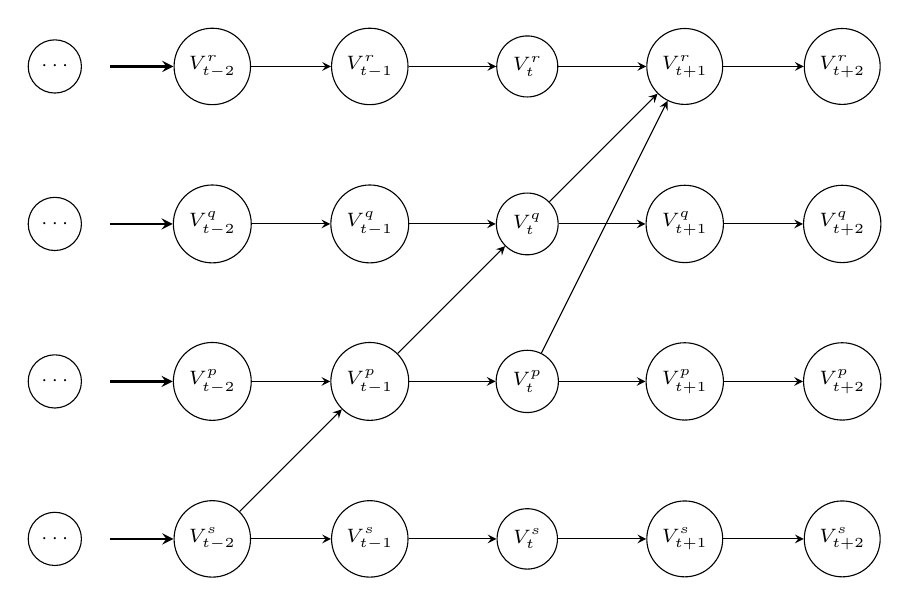
\begin{tikzpicture}[
    every node/.style={circle, draw, minimum size=0.5cm, font=\scriptsize},
    >=stealth,
    ->,
]

% Coordinates and ellipsis
\foreach \i/\y in {r/6, q/4, p/2, s/0} {
    % Main nodes from t-2 to t+2
    \foreach \j/\x in {-2/-4, -1/-2, 0/0, 1/2, 2/4} {
        \node (\i\j) at (\x,\y) {$V^{\i}_{t\ifnum\j<0 \j\else\ifnum\j=0 \else+\j\fi\fi}$};
    }
    % Dots on the far left
    \node at (-6,\y) {$\cdots$};
    % Arrows from dots to first node
    \draw[->, thick] (-5.3,\y) -- (\i-2);
}

% Temporal self-links
\foreach \i in {r,q,p,s} {
    \foreach \j/\k in {-2/-1, -1/0, 0/1, 1/2} {
        \draw (\i\j) -- (\i\k);
    }
}

% Cross-temporal causal edges
\draw (s-2) -- (p-1);
\draw (p-1) -- (q0);
\draw (q0) -- (r1);
\draw (p0) -- (r1);

\end{tikzpicture}
\caption{Full time causal graph: The temporal SCM extends infinitely into the past (indicated by \(\cdots\) and incoming arrows) and shows both auto- and cross-variable lagged dependencies. Notice that in this example, no causal stationarity is assumed.}
\label{fig:full-time-causal-graph}
\end{figure}

\begin{definition}[Full-Time Causal Graph]
Let \(\left\{ \mathbf{V}_t \right\}_{t \in \mathbb{Z}}\) be a multivariate stochastic process governed by a Temporal SCM. The \textit{full-time causal graph} is the infinite directed acyclic graph (DAG) whose nodes are all variables \(V^i_t\) for every \(i \in \{1, \dots, N\}\) and every time step \(t \in \mathbb{Z}\), and whose edges correspond to direct causal relationships \(V^i_{t - \tau} \rightarrow V^j_t\) as defined by the TSCM. This graph includes both within-variable (autoregressive) and cross-variable temporal dependencies across all lags up to \(\ell_{\max}\).
\end{definition}

Figure \ref{fig:full-time-causal-graph} illustrates such a structure, where both temporal self-dependencies and cross-variable influences are made explicit. This infinite graph represents the most faithful unfolding of the SCM in time. If causal stationarity is not assumed (as illustrated), then different causal graphs correspond to different time horizons, further complicating the causal discovery task. Secondly, the full-time causal graph can be truncated to a specific time-horizon, resulting in the \textit{time-lagged (also called \textit{windowed}) causal graph}, with causal edges up to \(\ell_\text{max}\). 

\begin{definition}[Lagged Causal Graph - Window Causal Graph]
A \textit{lagged causal graph} is a directed acyclic graph (DAG) that represents causal relationships between time-shifted variables in a multivariate time-series. Formally, let \(\mathbf{V}_t = \{V^1_t, V^2_t, \dots, V^k_t\}\) denote the set of observed variables at time step \(t\). A lagged causal graph \(\mathcal{G}\) contains directed edges of the form \(V^i_{t-\tau} \rightarrow V^j_t\), where \(\tau \in \{1, 2, \dots, \ell_{\max}\}\) is a positive time lag. An edge \(V^i_{t-\tau} \rightarrow V^j_t\) indicates that \(V^i\) is a direct cause of \(V^j\) with a time lag of \(\tau\).
\end{definition}

An example of a lagged causal graph is illustrated in Figure \ref{fig:temporal-graphs} (a). Finally, the lagged causal graph can be further simplified to a more concise representation, the \textit{summary causal graph}.

\begin{definition}[Summary Causal Graph]
 Given a lagged causal graph \(\mathcal{G}\) with edges of the form \(V^i_{t-\tau} \rightarrow V^j_t\) for various lags \(\tau\), the corresponding summary graph \(\mathcal{S}\) contains an edge \(V^i \rightarrow V^j\) if there exists at least one lag \(\tau\) such that \(V^i_{t-\tau}\) is a direct cause of \(V^j_t\) in \(\mathcal{G}\).
\end{definition}

Essentially, a summary graph is a simplified representation of the lagged causal structure in a time-series, where the temporal information about lags is abstracted away, as shown in Figure \ref{fig:temporal-graphs} (b). The summary graph collapses temporal information and only displays whether a causal relationship exists between two variables, but it does not specify the lag or delay at which the causal influence occurs. Note that from a lagged causal graph one can obtain the summary graph (e.g. from Figure \ref{fig:temporal-graphs} (a) to Figure \ref{fig:temporal-graphs} (b)), but not vice-versa, as the lag of causal relationships is not encoded in the summary structure. Summary graphs that retain temporal information can of course be obtained from the lagged causal graph, but remain outside the scope of our text.   

\begin{figure}[t!]
\centering

% Lagged and Summary Graph Side-by-Side
\begin{minipage}[t]{0.48\textwidth}
\centering
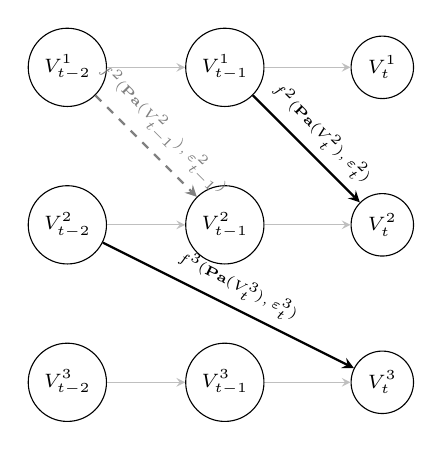
\begin{tikzpicture}[
    varnode/.style={circle, draw, minimum size=0.6cm, font=\scriptsize},
    >=stealth,
    ->,
    dashededge/.style={->, dashed, thick, color=gray},
    solidedge/.style={->, thick},
]

% t-2
\node[varnode] (V1t2) at (0,4) {$V^1_{t-2}$};
\node[varnode] (V2t2) at (0,2) {$V^2_{t-2}$};
\node[varnode] (V3t2) at (0,0) {$V^3_{t-2}$};

% t-1
\node[varnode] (V1t1) at (2,4) {$V^1_{t-1}$};
\node[varnode] (V2t1) at (2,2) {$V^2_{t-1}$};
\node[varnode] (V3t1) at (2,0) {$V^3_{t-1}$};

% t
\node[varnode] (V1t) at (4,4) {$V^1_{t}$};
\node[varnode] (V2t) at (4,2) {$V^2_{t}$};
\node[varnode] (V3t) at (4,0) {$V^3_{t}$};

% Optional: temporal arrows (light gray)
\foreach \i in {1,2,3} {
  \draw[->, gray!50] (V\i t2) -- (V\i t1);
  \draw[->, gray!50] (V\i t1) -- (V\i t);
}

% Causal arrows with functional labels directly on edges
\draw[solidedge] (V1t1) -- (V2t)
  node[midway, above, sloped, font=\tiny, draw=none, fill=none] 
  {$f^{2}(\mathbf{Pa}(V^2_t),\varepsilon^2_t)$};

\draw[dashededge] (V1t2) -- (V2t1)
  node[midway, above, sloped, font=\tiny, draw=none, fill=none] 
  {$f^{2}(\mathbf{Pa}(V^2_{t-1}),\varepsilon^2_{t-1})$};

\draw[solidedge] (V2t2) -- (V3t)
  node[midway, above, sloped, font=\tiny, draw=none, fill=none] 
  {$f^{3}(\mathbf{Pa}(V^3_t),\varepsilon^3_t)$};

\end{tikzpicture}


\vspace{0.5em}
{(a) Lagged causal graph}
\end{minipage}
\hfill
\begin{minipage}[t]{0.48\textwidth}
\centering
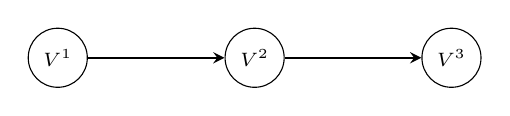
\begin{tikzpicture}[
    every node/.style={circle, draw, minimum size=0.6cm, font=\scriptsize},
    >=stealth,
    ->,
]

\node (V1) at (2,2) {$V^1$};
\node (V2) at (4.5,2) {$V^2$};
\node (V3) at (7,2) {$V^3$};

\draw[->, thick] (V1) -- (V2);
\draw[->, thick] (V2) -- (V3);

\end{tikzpicture}

\vspace{0.5em}
{(b) Summary causal graph}
\end{minipage}

\caption{Illustration of a temporal SCM with max lag \(\ell_{\max}=2\). (a) The lagged causal graph shows variable \(V^1\) causing \(V^2\) with lag 1, and \(V^2\) causing \(V^3\) with lag 2. Dashed edges encode the assumption of causal stationarity, meaning that the same causal dependencies recur over time. Functional dependencies between lagged variables are shown directly on edges. (b) The summary causal graph discards time lag information, representing only the aggregated causal influences.}
\label{fig:temporal-graphs}
\end{figure}

\section{Probabilistic Quantifications} \label{sec:bns}

To introduce our next causal assumptions, one needs to understand how causal structures relate to probabilistic reasoning, by the formalism of \textit{Bayesian networks (BNs)}. BNs provide a compact representation of a joint probability distribution using a directed acyclic graph. Each node corresponds to a random variable, and each directed edge represents a statistical dependence.

Briefly, a Bayesian network is defined as a pair \((\mathcal{G}, \mathbb{P})\), where \(\mathcal{G} = (\mathbf{V}, \mathcal{E})\) is a DAG with nodes \(\mathbf{V} = \{X_1, \dots, X_n\}\), and \(\mathbb{P}\) is a joint distribution over \(\mathbf{V}\), which factorizes, according to the chain rule, based on the structure of \(\mathcal{G}\). That is, each variable \(X_i\) is conditionally independent of its non-descendants given its parents \(\mathrm{Pa}(X_i)\) in the graph:

\begin{equation}
\mathbb{P}(X_1, \dots, X_n) = \prod_{i=1}^n \mathbb{P}(X_i \mid \mathrm{Pa}(X_i)).
\end{equation}

This factorization, which \citet{bengio2019meta} call \textit{disentangled factorization}, provides both computational efficiency and semantic clarity: each conditional distribution models a local dependency, and the global distribution emerges from their composition. Compared to SCMs which explicitly model causal mechanisms through assignments \(X_i := f_i(\mathrm{Pa}(X_i), \epsilon_i)\), BNs represent probabilistic dependencies only. While every SCM induces a Bayesian Network (through the distribution entailed by its noise and mechanisms), the converse does not hold; Bayesian Networks may not capture the directionality or manipulability implied by causality, so interventions and counterfactuals are not applicable. If one assumes causal interpretation on the edges, the resulting BN can be treated as a \emph{causal BN}. In a nutshell, the key advantage of Bayesian Networks lies in their ability to encode and reason about conditional independencies, which are central to many causal discovery approaches.


\section{Causal Assumptions} \label{sec:causal-assumptions}

We now elaborate on causal assumptions needed for performing identifiability of the true causal graph and consequently, sound causal inference. We have already elaborated on the assumption of causal stationarity in Section \ref{sec:temp-scms}. All causal discovery algorithms are governed by a set of assumptions, regarding the statistical properties of the data and the underlying causal structure. It is thus evident that making and understanding causal assumptions is also vital for correct interpretation not only of the discovered causal structure. We define the following assumptions in a way to be applied to either a (standard) causal graph or analogously to a temporal causal graph.

\begin{definition}[Causal Markov Condition, \citep{spirtes2001causation}] Let \(\mathcal{G}\) be a causal graph with vertex set \(\mathbf{V}\) and \(\mathbb{P}\) a probability distribution over \(\mathbf{V}\), generated by the causal structure induced by \(\mathcal{G}\). Then \(\mathcal{G}\) and \(\mathbb{P}\) satisfy the Markov Condition if and only if \(~\forall ~W \in \mathbf{V}\), \(W\) is independent of its non-descendants (non causal effects) given its parents (direct causes) on \(\mathcal{G}\).
\end{definition}

Essentially, the Causal Markov Condition assures that conditional independences between variables are exactly those entailed by the causal graph (i.e. by d-separation).

\begin{definition}[Faithfulness, \citep{spirtes2001causation}] Let \(\mathcal{G}\) be a causal graph and \(\mathbb{P}\) a probability distribution over \(\mathbf{V}\). We say that \(\mathcal{G}\) and \(\mathbb{P}\) are faithful to each other if and only if (iff) the all and only the independence relations of \(\mathbb{P}\) are entailed by the Causal Markov condition of \(\mathcal{G}\). Specifically, \(\mathcal{G}\) and \(\mathbb{P}\) satisfy the Faithfulness Condition if-f every conditional independence relation true in \(\mathbb{P}\) is entailed by the Causal Markov Condition applied to \(\mathcal{G}\).
\end{definition}

In other words, given a causally sufficient set of variables \(\mathcal{U}\) in a population \(N\), \textit{every} conditional independence relation that holds in the density over \(\mathcal{U}\) \textit{is entailed by the local directed Markov condition for the causal DAG of \(N\)}. The key argument behind assuming faithfulness of the true causal graph and the corresponding distribution induced by observed data is that non-faithfulness would lead to determinism in the observed system. As everything would cause everything and no stochasticity is involved, performing causal queries would prove invalid.  

\begin{definition}[Causal Sufficiency, \citep{spirtes2001causation}] A set \(\mathbf{V}\) of variables is causally sufficient for a population iff in the population every common cause of any two or more variables in \(\mathbf{V}\) is in \(V\), or has the same value for all units in the population. The common cause \(Z\) of two or more variables in a DAG \(X \leftarrow Z \rightarrow Y\) is called a \textit{confounder of \(X\) and \(Y\)}. Hence causal sufficiency implies no unobserved confounders. The notion of causal sufficiency is being used without explicitly mentioning the population.
\end{definition}

\begin{figure}[ht!]
\begin{multicols}{2}
	\begin{center}
		\begin{tikzpicture}[->,>=stealth,thick]
			% X -> L -> Y
			\node[draw, circle] (XLY1) {$X$};
			\node[draw, rectangle,right=of XLY1] (L1) {$L$};
			\node[draw, circle,right=of L1] (Y1) {$Y$};
			
			\draw[->] (XLY1) -- (L1);
			\draw[->] (L1) -- (Y1);
		\end{tikzpicture}
	\columnbreak

		\begin{tikzpicture}[->,>=stealth,thick]
			% X <-> Y
			\node[draw, circle] (XY1) {$X$};
			\node[draw, circle,right=of XY1] (Y1) {$Y$};
			
			\draw[->] (XY1) -- (Y1);
		\end{tikzpicture}
	\end{center}
\end{multicols}

\begin{multicols}{2}
	\begin{center}
		\begin{tikzpicture}[->,>=stealth,thick]
			% X <-> L <-> Y
			\node[draw, circle] (XLY2) {$X$};
			\node[draw, rectangle,right=of XLY2] (L2) {$L$};
			\node[draw, circle,right=of L2] (Y2) {$Y$};
			
			\draw[<-] (XLY2) -- (L2);
			\draw[<-] (L2) -- (Y2);
		\end{tikzpicture}
	
	    \columnbreak
	    
		\begin{tikzpicture}[->,>=stealth,thick]
			% X <-> Y
			\node[draw, circle] (XY2) {$X$};
			\node[draw, circle,right=of XY2] (Y3) {$Y$};
			
			\draw[<-] (XY2) -- (Y3);
		\end{tikzpicture}
	\end{center}
\end{multicols}

\begin{multicols}{2}
		\begin{center}
		\begin{tikzpicture}[->,>=stealth,thick]
			% X <-> L <-> Y
			\node[draw, circle] (XLY2) {$X$};
			\node[draw, rectangle,right=of XLY2] (L2) {$L$};
			\node[draw, circle,right=of L2] (Y2) {$Y$};
			
			\draw[->] (XLY2) -- (L2);
			\draw[<-] (L2) -- (Y2);
		\end{tikzpicture}
	\end{center}
    \columnbreak
	\begin{center}
		\begin{tikzpicture}[->,>=stealth,thick]
			% X <-> Y
			\node[draw, circle] (XY2) {$X$};
			\node[draw, circle,right=of XY2] (Y3) {$Y$};
			
		\end{tikzpicture}
	\end{center}
\end{multicols}

\begin{multicols}{2}
	\begin{center}
		\begin{tikzpicture}[->,>=stealth,thick]
			% X <-> L <-> Y
			\node[draw, circle] (XLY2) {$X$};
			\node[draw, rectangle,right=of XLY2] (L2) {$L$};
			\node[draw, circle,right=of L2] (Y2) {$Y$};
			
			\draw[<-] (XLY2) -- (L2);
			\draw[->] (L2) -- (Y2);
		\end{tikzpicture}
	\end{center}
	
	\columnbreak
	
	\begin{center}
		\begin{tikzpicture}[->,>=stealth,thick]
			\node[draw, circle] (XY2) {$X$};
			\node[draw, circle,right=of XY2] (Y3) {$Y$};
			\node at (0.9,0) {?};
		\end{tikzpicture}
	\end{center}
\end{multicols}
\caption{Illustrations for the presence of a hidden confounder \(L\) for two variables \(X,Y\), in the case of atemporal data. In the first case, where \(X\) indirectly causes \(Y\) with \(L\) acting as a mediator, we observe that \(Dep(X,Y)\) so we infer \(X \rightarrow Y\), and similarly \(X \leftarrow Y\) in the second case. In the third case where \(X\) and \(Y\) share a hidden common effect, we infer \(Indep(X,Y)\) and thus discover no edge between \(X\) and \(Y\). However, in the case of \(L\) being a hidden common cause of \(X\) and \(Y\), there exists no DAG that captures the dependencies.}
\label{fig:dag-conf}
\end{figure}

To put it simply, causal sufficiency is the \textit{assumption of no unobserved variables}. Unobserved variables are called \textit{latent} or \textit{hidden}. The fact that DAGs are unable to adequately capture latent confounders becomes apparent in the example at Figure \ref{fig:dag-conf}, for the case of i.i.d. data. The assumption can be adapted similarly for the case of time-series, where one can assume latent confounders may exist at a predefined time-lag. For example \(V^1_{t}\) and \(V^2_{t}\) may be confounded by the latent variable \(V^3_{t-1}\). SCMs without unobserved confounders are also called \textit{Markovian models} as the noise terms of the variables are independent. The observed variables in SCMs with unobserved confounding can have dependent noise terms, called \textit{semi-Markovian models}.

It must be noted that in practice, not all variables in the underlying SCM are measured. A projected causal graph on the observed subset is represented as an \textit{Acyclic Directed Mixed Graph} (ADMG), in which a bidirected arrow \(V^i_{t-\tau}\leftrightarrow V^j_t\) indicates the presence of an unobserved common cause with lag \(\tau\). For atemporal data, causal structures that enable marginalization of an SCM (a model with a subset of variables) exist \citep{richardson2002ancestral}, but remain completely outside our scope. This formulation also underlies algorithms for causal discovery under latent confounding, or when inferring contemporaneous effects where directionality is unknown.

\begin{figure}[h]
\centering
\begin{tikzpicture}[
    every node/.style={circle, draw, minimum size=0.6cm, font=\scriptsize},
    >=stealth,
    ->,
    solidedge/.style={->, thick},
    removededge/.style={->, red, dotted, thick, opacity=0.5},
    interbox/.style={rectangle, draw, minimum width=0.5cm, minimum height=0.4cm, font=\tiny, fill=black!5}
]

% Nodes at t-2
\node (V1t2) at (0,6) {$V^1_{t-2}$};
\node (V2t2) at (0,4) {$V^2_{t-2}$};
\node (V3t2) at (0,2) {$V^3_{t-2}$};

% Nodes at t-1
\node (V1t1) at (3,6) {$V^1_{t-1}$};
\node (V2t1) at (3,4) {$V^2_{t-1}$};
\node (V3t1) at (3,2) {$V^3_{t-1}$};

% Nodes at t
\node (V1t) at (6,6) {$V^1_{t}$};
\node (V2t) at (6,4) {$V^2_{t}$};
\node (V3t) at (6,2) {$V^3_{t}$};

% Temporal identity edges (gray)
\foreach \i in {1,2,3} {
  \draw[->, gray!50] (V\i t2) -- (V\i t1);
  \draw[->, gray!50] (V\i t1) -- (V\i t);
}

% Causal edges
\draw[->, gray!50] (V1t2) -- (V3t1);     % V^1_{t-2} -> V^3_{t-1}
\draw[solidedge] (V1t1) -- (V3t);        % V^1_{t-1} -> V^3_t
\draw[->, gray!50] (V2t2) -- (V3t1);     % V^2_{t-2} -> V^3_{t-1}
\draw[solidedge] (V2t1) -- (V1t);        % V^2_{t-1} -> V^1_t
\draw[solidedge] (V2t1) -- (V3t);        % V^2_{t-1} -> V^3_t

% Removed incoming edges to V1_{t-1}
\draw[removededge] (V1t2) -- (V1t1);     % V^1_{t-2} -> V^1_{t-1} (self-dependence, optional)
\draw[removededge] (V2t2) -- (V1t1);     % V^2_{t-2} -> V^1_{t-1}

% Intervention label
\node[interbox, right=2pt of V1t1] {\scriptsize do($V^1_{t-1}$)};

\end{tikzpicture}
\caption{A dense lagged causal graph with an intervention on \( V^1_{t-1} \), where \(V^2\) directly causes \(V^1\) \& \(V^3\) with lag 1 and \(V^1\) directly causes \(V^3\) with lag 1. The intervention \( \text{do}(V^1_{t-1}) \) removes all incoming edges to \( V^1_{t-1} \), shown as red dotted lines, while preserving its downstream influence on \( V^3_t \). The interventional value replaces the natural dynamics of \( V^1_{t-1} \), breaking any backdoor paths through its original causes.
}
\label{fig:interv-example}
\end{figure}

As we have seen in Chapter \ref{chap:introduction}, the first rung that differentiates a probabilistic model with a causal model is the ability to perform interventions, that is, modifying the internal causal mechanisms of the examined system. We define interventions for the temporal setting, which only differs in the temporal dimension of the variables. TSCMs allow interventions to be performed in a simple manner: Modify the structural assignment in the SCM of a variable \(X^k\) to \(x\). This corresponds to a \textit{hard intervention} at a specific timestep \(t\). The resulting interventional distribution \(\mathbb{P}(Y_t|\text{do}(X^k_t=x))\) captures the causal effect of setting \(X\) to \(x\). The reader should recall that the observational and interventional distributions may differ because non-causal associations (e.g., due to confounders) are blocked under interventions. In the causal graph, this corresponds to performing \textit{graph surgery}, by removing all incoming edges to \(X^k_t\) and replacing the structural equation with \(X^k_t:=x\), due to what is known as the \textit{modularity assumption}. An example is illustrated in Figure \ref{fig:interv-example}. One may also apply different interventions to different variables \(X^i_t, X^j_t\), (\textit{multiple interventional targets}) at the same timestep, resulting in an interventional distribution \( \mathbb{P}(Y_t | \text{do}(X^i_t=x^i_t, X^j_t=x^j_t))\). For soft interventions, as the name may suggest, instead of explicitly modifying the structural assignment, one adds a noise term (either sampled from a known parametric distribution like a Gaussian, or sampled from a prior distribution) to the structural assignment. Consequently, interventions allow us to define causality in a much more rigid manner: A variable \(X^i\) causes \(X^j\) if an intervention on \(X^i\) leads to a direct change in \(X^j\). Conclusively, do-calculus provides a set of transformation rules to express interventional (and counterfactual, although outside of our scope) distributions in terms of observable quantities, given a true or discovered causal graph. It underpins identification results, determining whether a causal effect can in principle be recovered from observational data alone or whether additional assumptions or interventional data are required. For causal discovery algorithms, handling of interventional data leads further into correct identifiability of the true causal graph, which may not be possible with observational data alone. 